% CPSC 438 Final Project Paper
% Christopher Chute, David Brandfonbrener, Leo Shimonaka, Matthew Vasseur

% Author and Title Information
\newcommand*{\thetitle}{Scalability Limits of HDFS}
\newcommand*{\theauthor}{Christopher Chute, David Brandfonbrener, Leo Shimonaka, Matthew Vasseur}
\newcommand*{\duedate}{May 3, 2016}

% Document Settings
\documentclass[11pt, a4paper]{article}
\author{\theauthor}
\title{\thetitle}
\date{\duedate}
\usepackage[top=.75in, left=0.5in, right=0.5in, bottom=1.5in]{geometry}
\usepackage{amsmath, amsthm, amssymb}
\newtheorem{lem}{Lemma}
\usepackage{graphicx}
\usepackage{setspace}
\usepackage{enumitem}
\usepackage{booktabs}
\usepackage[T1]{fontenc}
\usepackage{titling}

% Multicolumn Formatting
\usepackage{multicol}
\setlength\columnsep{18pt}    % spacing between columns

\setlength{\droptitle}{-9em}
\posttitle{\par\end{center}\vspace{-.35em}}

% Header Formatting
\usepackage{fancyhdr}
\setlength{\headheight}{48pt}
\pagestyle{fancyplain}
%\lhead{\thetitle}
%\rhead{\theauthor\\\duedate}
%\rfoot{}
\cfoot{\thepage}

% ************************* End of Preamble ***********************
\begin{document}
\maketitle
\thispagestyle{empty}

\begin{abstract}
    This paper explores the scalability limits of the Hadoop Distributed File System (HDFS). The single-machine, in-memory metadata store of HDFS is a known bottleneck for applications requiring storage of many small files. This architecture presents other theoretical bottlenecks, including CPU load on the NameNode from storing many small files. For example, both high-frequency requests and heartbeats with small files require higher NameNode CPU usage. In this paper we model and provide experimental evidence for the NameNode memory bottleneck. We compare this to proposed CPU bottlenecks, and we find that the memory bottleneck is the dominant issue. We provide suggestions for future work on HDFS scalability limits.
\end{abstract}
\begin{multicols*}{2}


\section{Introduction}

Distributed filesystems (DFS), also known as network filesystems, stores remote files in a format accessible with the same semantics as a local filesystem. It offers a transparent interface for handling files and directories, abstracting features like access control, recovery and concurrency. DFS offers a scalable mechanism for creating logical filesystems shared by many clients.

The DFS architecture has many advantages; it offers a unified hierarchical namespace for shared files and folders, location transparency in physical data placement, load balancing across nodes, storage scalability via expanding clusters, increased availability through distributed data, and fault tolerance by replication across racks.

Many DFS implementations exist today. Each system differs in their performance, data mutability, handling of concurrent writes, failure handling, and storage policies. These include POSIX-compliant systems like Lustre, search-engine enhanced Google File System (GFS), and non-proprietary open-source DFSs like Hadoop Distributed File System.

This paper examines Hadoop Distributed File System (HDFS), a module of the Apache Hadoop ecosystem. HDFS is a distributed filesystem focused on scalability and portability. HDFS is not fully POSIX-compliant since it is specifically designed for handling large files terabytes in size. It trades the POSIX functionality like mutable files for increasing data throughput and supporting operations like Append.

The architecture of HDFS is designed with the following goals in mind:
\begin{enumerate}[noitemsep, label=\arabic*.]
	\item\textit{Support regular hardware failure.} This is accomplished primarily through replication of data across multiple DataNodes.
	\item\textit{Allow streaming data access.} Partitioning should be transparent so that files appear to be stored sequentially. Reads are distributed so that streaming access does not block other transactions.
	\item\textit{Support very large data sets.} To provide scalability, more DataNodes can be added to support large data sets. This assumes that the NameNode memory limit will not become a bottleneck before the disk space of the DataNodes.
	\item\textit{Provide simple concurrency control.} The write-once, read-many model mainly accomplishes this. Only appends are allowed, and only one appender/creator per file is allowed at once. This allows HDFS to provide highly available and concurrent reads.
	\item\textit{Run everywhere (portability).} HDFS runs on top of the Java Virtual Machine, which provides nearly universal portability.
\end{enumerate}

HDFS's key characteristic is in how it decouples metadata from file data. Although its centralized namespace storage offers several advantages for linear performance scaling, it also introduces hard bounds for growth. This paper explores how these limitations occur, analyzes its objective effects on performance, and discusses potential approaches to overcoming this limit.

The rest of this paper is organized as follows. In section 2, we outline the architecture of a HDFS cluster. Section 3 provides a high-level overview of how this architecture interferes with the system's performance. Section 4 discusses the design and analysis of various experiments conducted on an HDFS cluster, followed by proposals on ways to improve performance in Section 5.
% -------------------------------------------------

\section{HDFS Architecture}
% TODO: Figures?

With these principles in mind, the HDFS architecture is designed as follows. An HDFS cluster consists of a single NameNode and many DataNodes. Briefly, the NameNode holds the metadata for each file in the file system. Metadata for a directory consists of an inode, and metadata for a file consists of an (inode, mapping) pair. The inode is a UNIX-style inode and thus contains properties such as permissions and ownership. Moreover, an HDFS inode stores HDFS-specific attributes such as quotas and replication factors.

% TODO: Say which section the linear block result is presented in.
Each file is partitioned into one or more blocks, and each block is replicated across multiple DataNodes. The mapping for a file maps each block of the file to a list of DataNodes where the block is replicated. As presented below, the metadata associated with each file scales linearly with the number of blocks in each file. That is, there is a fixed size mapping for each block in the file. The NameNode holds all of this metadata in memory to facilitate fast metadata operations.

A single NameNode is used primarily to simplify the architecture and metadata management of HDFS. For instance, having a single NameNode makes it simpler to maintain consistency in the file system. A single NameNode architecture also allows for simple, centrally organized replication of each block across many DataNodes. If the metadata was not centralized, this replication operation and updating all data mappings would become complicated, and potentially overuse the network connecting the nodes.

All metadata is kept in memory on the NameNode. Given a file of size $F$ and a block size $B$, the file will be partitioned into $n = \lceil F/B\rceil$ blocks. Upon creation of the file, the NameNode replicates each of the $n$ blocks across $R$ DataNodes, where $R$ is the \textit{replication factor} of the cluster. Once the file is created, the NameNode is responsible for pointing read or append requests to the appropriate blocks on the DataNodes. The NameNode keeps the block mappings up-to-date by communicating with the DataNodes via \textit{block reports} carried in periodic heartbeats from each DataNode. A heartbeat also indicates that a DataNode is functioning correctly and has a working network connection. The NameNode uses this information to ensure each block is replicated over $R$ DataNodes, issuing replication commands if needed.

Durability of the NameNode is critical to the availability of HDFS. There are various schemes to ensure a durable NameNode. A write-ahead log is maintained on stable storage and this can be used to build a BackupNode or CheckpointNode that essentially maintains a copy of the NameNode. By default, the NameNode is a single point of failure for an HDFS cluster, and reconstructing the NameNode after failure involves sending 

Files in HDFS are append-only and can only be written to by a single writer at a time so that once data is written it cannot be overwritten. This simplifies concurrency control and allows the system to guarantee that writes can be read as soon as a file is closed. On a write, a client must first query the NameNode to find which DataNodes and blocks to write. Then, the client will ensure a replicated write by sending packets of data through a pipeline of TCP connections. This pipeline includes all DataNodes over which the file will be replicated, which guarantees that the writes will be consistent across multiple DataNodes. On a read, a client must first query the NameNode to find which DataNodes contain replicas of the desired file and which blocks hold the file. Then, the client reads from the closest available DataNodes directly.

\section{Limitations of Single-NameNode Architecture}

Despite the benefits of having only a single NameNode, this architectural decision causes some potentially major scalability problems. These problems will be especially pronounced when HDFS is used to store many small files as opposed to few large files. In particular, small files produce more metadata relative to their content size, which quickly exhausts the available memory of the NameNode.

\subsection{Physical Memory Size}
% Re-iterate in-memory metadata namespace
% Total File Capacity of Cluster is Limited by Name Node's RAM due to requirement that all metadata objects (file inodes and block) in memory at all times
% SVENCHO PAPER EXAMPLE: Assuming on average, a file consists of \lambda = 1.5 blocks, then each file uses 1 file and ~2 data block objects, hence uses ~600 bytes. Thus to keep 100 million files, name-node must have at least 60GM of RAM

The obvious problem with forcing all metadata to be in memory on the NameNode is that the NameNode will run out of available memory. %todo cite Shvanko

Let $ M $ be the size of memory on the NameNode in bytes, $ \lambda $ be the number of blocks allocated to each file, and $ F $ be the number of files on the system. Also, let $ c $ be the number of bytes to represent a single block mapping to all replicas of a block, and $i$ the number of bytes to represent and inode. If we want to fit all metadata into memory, it is clear that we must have:
\begin{align*}
	M > \lambda c F + i F
\end{align*}
	This limit is much easier to reach with small files since each file is allocated its own virtual block, no matter how small the file is, i.e. we have that $ \lambda \geq 1$. This means that creating many small files should take up $ c + i$ bytes for each additional file, while growing a file by a similar amount will use at most $ c $ bytes. Thus, the memory limit is much more of a problem for many small files. 
	
	Using this model, we can perform simulations of how much data can be stored in an HDFS cluster if each file is of a given size. The motivation for this is that with larger files, each file will use more blocks, and thus create more metadata. However, the cost of storing the inode relative to the amount of data in the file will decrease with larger files. It is interesting to see how both file size and block size effect the total amount of data that an HDFS cluster can store before the memory bottleneck is reached.
	
	Below, we have graphs that represent the outcomes of these simulations. We assume that (like in our HDFS cluster on AWS) that the NameNode has 2GB of RAM, and perform the simulation for various block sizes (the size of each block that a file is divided into). We use the metadata sizes from our experimental section below of $ c = i = 150$. First, we ran the simulation with a block size of 128 MB. We have one plot of file sizes from 1 byte to 100 GB and another showing only file sizes larger than the block size of 128 MB, since this part is nonlinear and more interesting. 
	


\begin{center}
	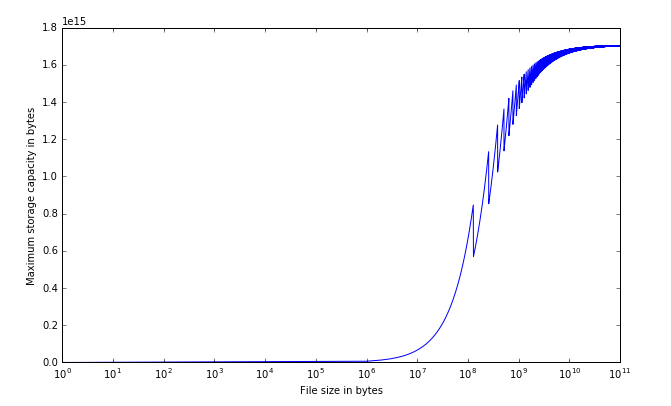
\includegraphics[keepaspectratio=true, width=0.45\textwidth]{logScale}	
\end{center}

\begin{center}
	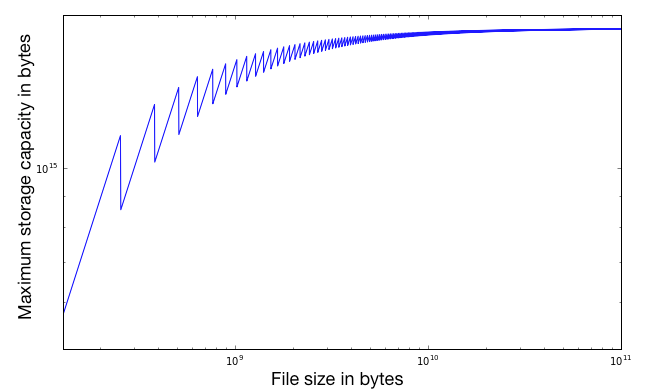
\includegraphics[keepaspectratio=true, width=0.45\textwidth]{logLogScale}	
\end{center}

While each file is smaller than one block, a file is always allocated its own block in the system and thus has a constant metadata size. Then, since the files are linearly increasing in the amount of data they hold, but metadata remains constant, the capacity of the system (as limited by the RAM on the NameNode) grows linearly until files are larger than blocks. 

Once a file is large than a block, the behavior becomes more interesting. Once the files get large enough to force an extra block to be allocated for each file, the cost of the extra metadata to record this block outweighs the increase in file size so that the overall capacity of the system decreases. This causes the zig-zag nature of the above graph. At the same time, the system also begins to reach the limit  

Lastly, we ran the same simulation with many different block sizes.  Since the size of each block directly effects how many blocks a file of a given size is split into, and thus how much metadata it has, a larger block size should create less metadata per file. This resulted in the following plot:
	
\begin{center}
	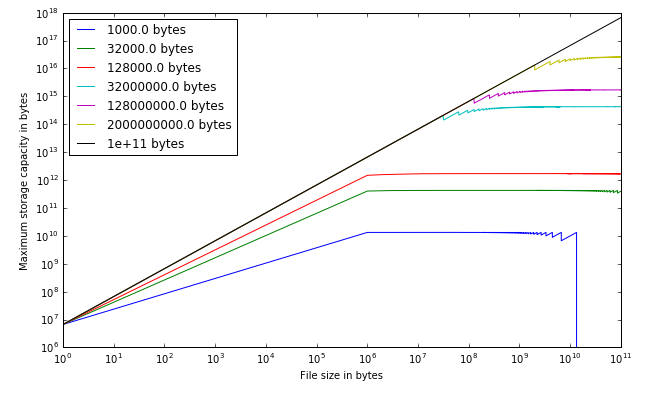
\includegraphics[keepaspectratio=true, width=0.45\textwidth]{variableBlockSize}	
\end{center}

This graph shows how larger block size does indeed lead to larger system capacity. 
(COST OF LARGER BLOCKS)

	CONCLUSIONS
	Thus, we expect this memory limit to be effected in the following main ways. (1) 

\subsection{Namenode CPU Bottleneck}
The less obvious scalability problem with the HDFS architecture is the potential for a CPU bottleneck at the NameNode. The system is built on the assumption that the NameNode operations are small enough and there will be few enough large files that they will be insignificant. However, with many small files, these assumptions are violated and the NameNode CPU could become a bottleneck. 

% Describe the INTERNAL-LOAD communicating with DataNodes
% # of Heartbeats that NameNode receives is directly proportional to # of DataNodes in cluster
% # of Block reports is also directly proportional to size of data blocks (i.e. ratio of blocks mapped per file) and also # of replicated copies per block
% Physical data storage and data I/O performance increase proportionally to # of DataNodes in cluster and size of data blocks, but the overall performance of HDFS is also affected negatively by increased internal load.
% The more time spend on internal load, less time spend on processing external client's requests

The first potential source of CPU bottleneck is the internal-load of communication with the DataNodes. This internal-load can be created in two ways. First, internal-load can be created when the system holds a large amount of small files. The size of the block report sent by each DataNode is directly proportional to the number of blocks that the DataNode holds. Since each file is given its own virtual block, even if the file is much smaller than a block, the DataNode can potentially hold a great number of small files and have to send a large block report containing the metadata of each of these files. This could potentially overload the NameNode CPU. 
Second, the number of block reports that a NameNode receives is directly proportional to the number of DataNodes in the system. So, if the system has a large number of DataNodes, it is possible to generate a large amount of internal load by having many DataNodes.  


% Describe the external-load from clients
% All metadata operations run on Namenode - they cannot be processed anywhere else.
% On every file read, there is a get_block_location per block per file
% On every file write, there is a create_block per block per file
% Namenode can become a bottleneck with operations that involve many metadata operations, e.g. batch-write operations will include many create_block requests

% -------------------------------------------------

Another potential source of CPU bottleneck is external-load from clients querying the NameNode. As explained above, on both reads and writes a client must first contact the NameNode to find the appropriate block locations and then the DataNodes for the read or write. Afterwards the NameNode must perform a metadata operation to determine what to return to the client. Therefore, the NameNode can become a bottleneck if there are many clients trying to perform operations concurrently since they all must access the metadata via the singular NameNode. This should be an especially prevalent problem when there are many small files because it would be likely that the use pattern of a system with many small files would be for there to be many clients each trying to access their files concurrently. 

With these potential CPU bottlenecks in mind, we pose the question of whether it is possible to generate an appropriate load so as to reach these CPU bottlenecks before the NameNode runs out of memory. This will be addressed by our experimentation. 

\section{Performance Evaluation}

% Discuss goals of tests (i.e. "we want to test Memory and CPU and determine blah")

% Mention experimental setup (EC2, Java Test Skeleton, # nodes, etc)

% FOR EACH EXPERIMENT:
% Discuss designs of individual experiments and their results
% What were the experiments testing?
% What were the different parameters of the experiments?
% Possibilities of error?

\subsection{Experiment 1: Memory Experiments}

% TODO: See above

\subsection{Experiment 2: CPU Experiments}

% TODO: See above

\subsection{Analysis}

% Discuss raw results independently for each experiment:
% Are these results what was expected (and why)?
% If there was some error, discuss what may have caused it
% Graphs

% Evaluate experimental results holistically to pinpoint the problem with HDFS's Single Namenode architecture (I.e. weigh CPU and Memory problems against each other)

% -------------------------------------------------

\section{Improvements to Single NameNode Architecture}

% Use experimental data to determine what is actually detrimental to performance of HDFS, and suggest a way to improve it

% -------------------------------------------------

% Would it be helpful to remove the assumption that each file is assigned to its own block? Could be done with intermediate layer that puts small files into larger file, prevents edits

% 

% mention HDFS federation, CalvinFS
% 

\section{Conclusion}

% Wrap it up with stuff.



%TODO sources

\end{multicols*}
\end{document}


























 ``